\documentclass[prb,12pt]{revtex4-2}

\usepackage{amsmath, amssymb,physics,amsfonts,amsthm}
\usepackage[most]{tcolorbox}
\usepackage{enumitem}
\usepackage{cancel}
\usepackage{booktabs}
\usepackage{polynom}
\usepackage{tabularx}
\usepackage{tikz}
\usepackage{hyperref}
\usepackage{enumitem}
\usepackage[normalem]{ulem}
\usepackage{transparent}
\usepackage{caption}
\usepackage{float}
\usepackage{multirow}
\newtheorem{Theorem}{Theorem}
\newtheorem{Proposition}{Theorem}
\newtheorem{Lemma}[Theorem]{Lemma}
\newtheorem{Corollary}[Theorem]{Corollary}
\newtheorem{Example}[Theorem]{Example}
\newtheorem{Remark}[Theorem]{Remark}
\theoremstyle{definition}
\newtheorem{Problem}{Problem}
\theoremstyle{definition}
\newtheorem{Definition}[Theorem]{Definition}
\newenvironment{parts}{\begin{enumerate}[label=(\alph*)]}{\end{enumerate}}
%tikz
\usetikzlibrary{patterns}
\usetikzlibrary{matrix}
%tcolorbox
\tcbset{breakable=true,toprule at break = 0mm,bottomrule at break = 0mm}
% definitions of number sets
\newcommand{\N}{\mathbb{N}}
\newcommand{\R}{\mathbb{R}}
\newcommand{\Z}{\mathbb{Z}}
\newcommand{\Q}{\mathbb{Q}}
\newcommand{\C}{\mathbb{C}}
\allowdisplaybreaks
\setlength{\parindent}{0cm}
\captionsetup[table]{name=Tabelle}

\begin{document}
\title{Versuch 29}
	\author{Jun Wei Tan}
	\email{jun-wei.tan@stud-mail.uni-wuerzburg.de}
	\affiliation{Julius-Maximilians-Universit\"{a}t W\"{u}rzburg}
	\date{\today}
	\maketitle

\section{Bestimmung von Wechselstromwiderstände durch Messung mit dem Oszillograph}
\subsection{Allgemeines}
Die Phasendifferenz ist definiert durch
\[\Delta\varphi=2\pi\frac{\Delta t}{T}\]
Am häufigsten brauchen wir die Phasendifferenz in Einheiten von $\pi$, also wir berechnen stattdessen
\[\frac{\Delta \varphi}{\pi}=\frac{2\Delta t}{T}\]
Dies kann ausgedrückt werden durch die Frequenz
\[\frac{\Delta \varphi}{\pi}=2(\Delta t)f\]
und der Fehler ist nach Gauß
\[\Delta \left(\frac{\Delta \varphi}{\pi}\right)=2\sqrt{f^2 [\Delta(\Delta t)]^2+(\Delta t)^2 (\Delta f)^2}\]
Wenn wir einen Mittelwert aus unterschiedliche Werte bilden, werden wir einen gewichteten Mittelwert verwenden
\[\bar{x}= \frac{\sum \frac{x_i}{\sigma_i^2}}{\sum \frac{1}{\sigma_i^2}}\]
und
\[\Delta \bar{x}=\frac{1}{\sqrt{\sum \frac{1}{\sigma_i^2}}}\]
\subsection{Ohmscher Widerstand}
Es ist
\[R=\frac{U_{pp,CHII}}{U_{pp,CHI}}R_{vor}\]
und daher nach Gauß
\[\Delta R = R\sqrt{\left(\frac{\Delta {U_{pp,CHI}}}{U_{pp,CHI}}\right)^2 + \left(\frac{\Delta {U_{pp,CHII}}}{U_{pp,CHII}}\right)^2+\left(\frac{\Delta R_{vor}}{R_{vor}}\right)^2}\]
Der Vorwiderstand ist nach Produktbeschreibung
\[R_{vor}=(6,85\pm 0,17)~\text{k}\Omega\]
\begin{center}                                                                         
 \begin{tabular}{ccc}
 	\toprule
 	$f$ (Hz) & $100,0\pm 1,1$ & $1000\pm 11$\\\midrule
 	$U_{pp,CHI}$ & $(14,00\pm 0,40)$ V & $(14,00\pm 0,40)$ V\\\midrule
 	$U_{pp,CHII}$ & $(3,70\pm 0,10)$ V & $(3,70\pm 0,10)$ V\\\midrule
 	$R~(\Omega)$ & $(1,810\pm 0,084)~\text{k}\Omega$ & $(1,810\pm 0,084)~\text{k}\Omega$\\\midrule
 	Abstand zwischen Maxima & $(0\pm 50)~\mu$s & $(0\pm 50)~\mu$s\\\midrule
 	Phasendifferenzen & $(0,000\pm 0,010)\pi$ & $(0,00\pm 0,10)\pi$\\\bottomrule
 \end{tabular}
\end{center}

Dann bilden wir den Mittelwert
\[R=(1,810\pm 0,059)~\text{k}\Omega\]
Die Phasendifferenz ist
\[\Delta \varphi=(0,000\pm 0,010)\pi\]
\subsection{Kondensator}
Der Vorwiderstand ist
\[R=(226,4\pm 3,9)~\Omega\]
\begin{center}
	\begin{tabularx}{\textwidth}{XXXXXX}
	\toprule
	$f$ (Hz) & $100,0\pm 1,1$ & $500,0\pm 3,9$ & $1000\pm 11$ & $5000\pm 39$ & $10000\pm 110$\\\midrule
	$U_{pp,CHI}$ (V) & $1,160\pm 0,040$ & $4,00\pm 0,10$ & $4,80\pm 0,20$ & $4,40\pm 0,20$ & $5,20\pm 0,20$ \\\midrule
	$U_{pp,CHII}$ (V) & $19,0\pm 1,0$ & $12,40\pm 0,40$ & $7,60\pm 0,20$ & $1,70\pm 0,10$ & $0,820\pm 0,040$\\\midrule
	$R~(\Omega)$ & $3710\pm 240$ & $702\pm 31$ & $358\pm 19$ & $87,5\pm 6,7$ & $35,7\pm 2,3$\\\midrule
	Abstand zwischen Maxima ($\mu$s) & $2500\pm 200$ & $500\pm 50$ & $260\pm 20$ & $50,0\pm 5,0$ & $25,0\pm 2,0$\\\midrule
	Phasendifferenz / $\pi$ & $0,500\pm 0,040$ & $0,500\pm 0,050$ & $0,520\pm 0,040$ & $0,500\pm 0,050$ & $0,500\pm 0,040$\\\bottomrule
\end{tabularx}
\end{center}
Das Plot von $R_L$ in Abhängigkeit von $f$ ist
\begin{center}
	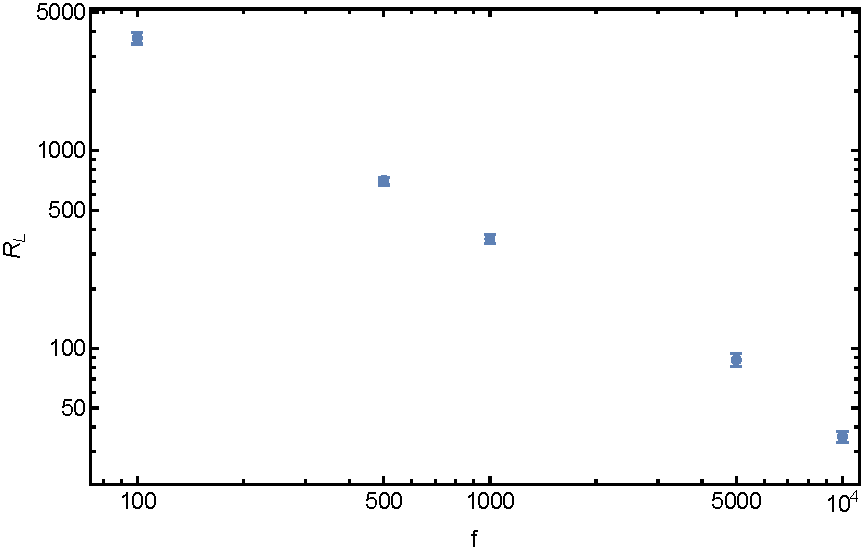
\includegraphics[width=	\textwidth]{plt1.pdf}
\end{center}
\subsection{Induktivität}
Der Vorwiderstand ist
\[R=(14,80\pm 0,54)~\Omega\]
Der Spulwiderstand ist
\[R_{Sp}=(2,40\pm 0,34)~\Omega\]
Wir berechnen den Scheinwiderstand analog wie vorher. Ferner brauchen wir
\[R_L=\sqrt{R_z^2 - R_{Sp}^2}\]
Dessen Fehler ist gegeben durch
\[\Delta R_L=\sqrt{\frac{R_z^2}{R_z^2 - R_{sp}^2}(\Delta R_z)^2+\frac{R_{Sp}^2}{R_z^2 - R_{sp}^2}(\Delta R_{Sp})^2}\]
\begin{center}
	\begin{tabularx}{\textwidth}{XXXXXX}
	\toprule
	$f$ (Hz) & $100,0\pm 1,1$ & $500,0\pm 3,9$ & $1000\pm 11$ & $5000\pm 39$ & $10000\pm 110$\\\midrule
	$U_{pp,CHI}$ (V) & $0,460\pm 0,020$ & $0,450\pm 0,020$ & $0,440\pm 0,020$ & $0,400\pm 0,010$ & $0,310\pm 0,010$ \\\midrule
	$U_{pp,CHII}$ (V) & $0,200\pm 0,010$ & $0,920\pm 0,040$ & $1,80\pm 0,10$ & $8,40\pm 0,40$ & $13,02\pm 0,40$\\\midrule
	$R_z~(\Omega)$ & $6,43\pm 0,49$ & $30,3\pm 2,2$ & $60,5\pm 4,9$ & $311,\pm 20,$ & $622,\pm 36,$\\\midrule
	$R_L~(\Omega)$ & $5,97\pm 0,54$ & $30,2\pm 2,2$ & $60,5\pm 4,9$ & $311,\pm 20,$ & $622,\pm 36,$\\\midrule
	Abstand zwischen Maxima ($\mu$s) & $2800\pm 200$ & $475\pm 50$ & $260\pm 20$ & $50,0\pm 5,0$ & $24,0\pm 2,0$\\\midrule
	Phasendifferenz / $\pi$ & $0,560\pm 0,040$ & $0,475\pm 0,050$ & $0,520\pm 0,040$ & $0,500\pm 0,050$ & $0,480\pm 0,040$\\\bottomrule
\end{tabularx}
\end{center}
Das Plot von $R_L$ in Abhängigkeit von $f$ ist
\begin{center}
	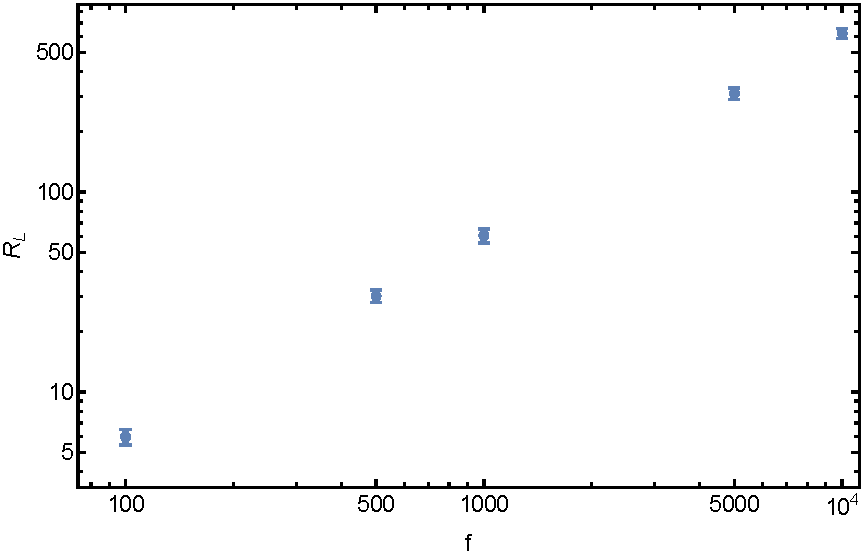
\includegraphics[width=	\textwidth]{plt2.pdf}
\end{center}
\end{document}
